\definecolor{bg}{rgb}{0.95,0.95,0.95}
\chapter{دستور کار آزمایش ها}

\section{کار با پایه های ورودی خروجی به روش های سرکشی و وقفه محور}

\subsection{اهداف آزمایش}
\begin{itemize}
    \item آشنایی با \lr{GPIO}
    \item آشنایی با روش های سرکشی و وقفه محور برای مدیریت \lr{Peripheral} های جانبی
    \item مقایسه‌ی دو روش سرکشی و وقفه محور
\end{itemize}

\subsection{قطعات مورد نیاز}

\begin{itemize}
    \item بورد \lr{Arduino Uno}
    \item دیود نورانی \lr{LED}
    \item کلید \lr{Switch}
    \item مقاومت ۲۲۰ اهم
    \item مقاومت ۱۰ هزار اهم
\end{itemize}
\pagebreak

\subsection{مقدمه}

\begin{nas} دو تابع اصلی در برنامه‌نویسی آردوینو \end{nas}
\newline
محیط آردوینو برای راحت تر شدن برنامه‌نویسی ۲ تابع مهم در اختیار ما می‌گذارد. نام این دو تابع \lr{begin} و \lr{loop} است.
\newline
\textcolor{red}{\begin{nas}سوال: \end{nas}}
در مورد این دو تابع تحقیق کنید و بنویسید که هر کدام در چه زمانی اجرا می‌شوند.

\newline
\begin{nas}دیود نوری
\end{nas}
\newline
دیود های نوری نوعی دیود هستند که هنگام عبور جریان از پایانه‌ی مثبت به پایانه‌ی منفی آنها، از خود نور ساتع می‌کنند. خواص الکتریکی دیود های نوری مشابه با دیود های دیگر است. این یعنی می‌توان یک دیود نوری روشن را به صورت یک منبع ولتاژ مدل سازی کرد. همچنین جریان عبوی از دیود های نوری دارای یک محدودیت است و اگر جریان بیشتر شود دیود نوری می‌سوزد و به همین دلیل باید در مدار شامل دیود نوری یک مقاومت حدودا ۲۲۰ اهمی قرار دهیم. معمولا ولتاژ دیود های نوری بین ۲ تا ۳ ولت و یک جریان مناسب و به دور از خطر برای آنها ۲۰ میلی‌آمپر است. برای اینکه بفهمیم مقدار ۲۲۰ اهم از کجا آمده، مدار زیر را در نظر بگیرید.
\begin{figure}[h]
    \centering
    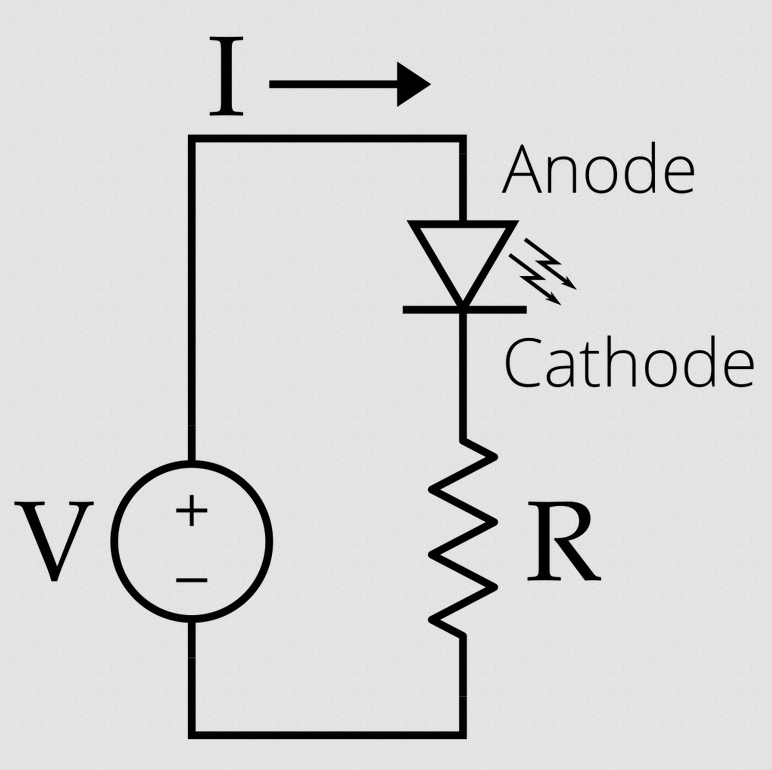
\includegraphics[width=8cm]{LED-Circuit.png}
    \caption{مدار دیود نوری}
    \label{fig:led-circ}
\end{figure}
\newline
\textcolor{red}{\begin{nas}سوال: \end{nas}}
با فرض اینکه ولتاژ دیود ۲ ولت باشد و منبع ولتاژ ۵ ولتی باشد، مقدار مقاومت سری را به گونه‌ای بیابید که جریان مدار ۱۵ میلی‌آمپر شود.
\newline
توجه کنید که دیود های نوری دو پایه دارند و پایه‌ای که بلند تر است پایانه‌ی مثبت دیود (آنود) و پایه‌ای که کوتاه تر است پایانه‌ی منفی (کاتود) دیود است. به هیچ عنوان دیود های نوری را به صورت برعکس در مدار قرار ندهید.
\pagebreak
\newline
\begin{nas}اتصال صحیح کلید به بورد\end{nas}
\newline
مدار زیر را در نظر بگیرید.
\newline
\begin{figure}[h]
    \centering
    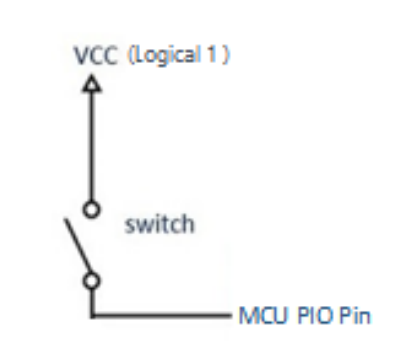
\includegraphics[width=8cm]{Switch-Direct.png}
    \caption{اتصال مستقیم کلید}
    \label{fig:swtch-dir}
\end{figure}
\newline
\textcolor{red}{\begin{nas}سوال: \end{nas}}
اگر کلید باز باشد ولتاژ \lr{MCU PIO Pin} چیست؟ این اتفاق چه مشکلی را پیش می‌آورد؟
\newline
برای حل مشکل مدار قبلی، باید از مقاومت های \lr{Pull Up} و \lr{Pull Down} استفاده کنیم. همانطور که از اسامی آنها پیداست، این مقاومت ها در هنگام قطع بودن کلید، ولتاژ را به بالا و یا به پایین می‌کشند. مدار های زیر را در نظر بگیرید:
\newline
\begin{figure}[h]
    \centering
    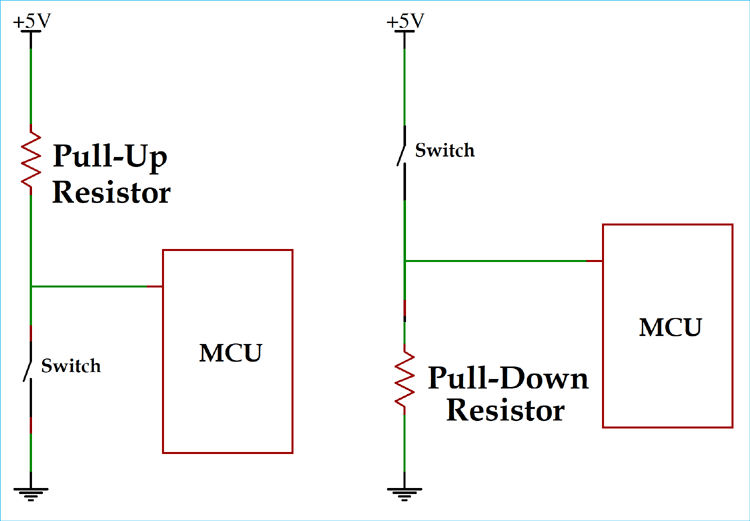
\includegraphics[width=8cm]{PUP-PDOWN.png}
    \caption{اتصال کلید با مقاومت های \lr{Pull Up} و \lr{Pull Down}}
    \label{fig:swtch-dir}
\end{figure}
\newline
\textcolor{red}{\begin{nas}سوال: \end{nas}}
ولتاژ ورودی به میکروکنترلر را در هر یک از مدار های بالا در حالت بسته و یا باز بودن میکروکنترلر محاسبه کنید.
\newline
\textcolor{red}{\begin{nas}سوال: \end{nas}}
بهتر است مقدار مقاومت استفاده شده مقدار بالایی باشد. دلیل این کار چیست؟
\newline
در نتیجه همواره برای اتصال یک کلید به میکروکنترلر از یکی از روش های \lr{Pull Up} و یا \lr{Pull Down} استفاده می‌کنیم.
\newline



\begin{nas}ورودی و خروجی\end{nas}
\newline
استفاده از پین های ورودی و خروجی از محیط آردوینو بسیار ساده‌است و با صدا زدن چند تابع انجام می‌شود.
\newline
\textcolor{red}{\begin{nas}سوال: \end{nas}}
در مورد توابع زیر تحقیق کنید و ورودی و خروجی هر تابع و کاری که انجام می‌دهند را بنوسید.
\begin{itemize}
    \item \lr{pinMode}
    \item \lr{digitalRead}
    \item \lr{digitalWrite}
    \item \lr{delay}
\end{itemize}




\begin{nas}وقفه\end{nas}
\newline
با وقفه ها در کلاس درس آشنا شدید. در سطوح پایین تر و نزدیک به سخت‌افزار به دلیل متفاوت بودن میکروکنترلر مورد استفاده در آزمایشگاه و میکروکنترلری که در کلاس درس تدریس شد، استفاده از وقفه ها مقداری متفاوت است اما به صورت کلی فرایند همان است.
\newline
\textcolor{red}{\begin{nas}سوال: \end{nas}}
انواع رویداد های ورودی که میکروکنترلر موجود در بورد \lr{Arduino Uno} می‌تواند تشخیص دهد و اعلام وقفه کند بنویسید.
\newline
\textcolor{red}{\begin{nas}سوال: \end{nas}}
کدام یک از پین های بورد شما قابلیت تشخیص وقفه را دارند؟
\newline
در محیط آردوینو استفاده از وقفه های مربوط به پین ورودی با استفاده از تابع \lr{attachInterrupt} صورت می‌گیرد.
\newline
\textcolor{red}{\begin{nas}سوال: \end{nas}}
در مورد تابع \lr{attachInterrupt} تحقیق کنید و ورودی و خروجی تابع و کاری که انجام می‌دهد را بنویسید.

\subsection{شرح آزمایش}

می‌خواهیم با استفاده از دیود نوری و کلید، یک شمارنده‌ی ۴ بیتی بسازیم. برای این کار، یک کلید را به همراه مقاومت \lr{Pull Up} یا \lr{Pull Down} به بورد متصل کنید و ۴ دیود نوری را نیز به هر یک از پین های بورد وصل کنید. فراموش نکنید که مقاومت سری ۲۲۰ اهمی را در مدار دیود های نوری قرار دهید.
سپس برنامه‌ای بنویسید که با استفاده از این ۴ دیود نوری از ۰ تا ۱۵ به صورت باینری شمارش کند و با هر بار فشردن کلید، یکی به عدد نمایش داده شده اضافه شود. برنامه را ابتدا به روش سرکشی و سپس به روش وقفه‌محور بنویسید.
\begin{itemize}
    \item به نظر شما اگر برنامه‌ی ما می‌خواست چند کار دیگر را نیز انجام دهد و شمردن با دیود نوری فقط یکی از وظایف آن بود، بهتر بود از کدام روش استفاده می‌کردیم؟
    \item اگر دکمه را برای مدت طولانی نگه دارید چه اتفاقی می‌افتد؟ دلیل این اتفاق چیست؟ برای حل این مشکل چه راه حلی دارید؟
\end{itemize}

\begin{figure}[h]
    \centering
    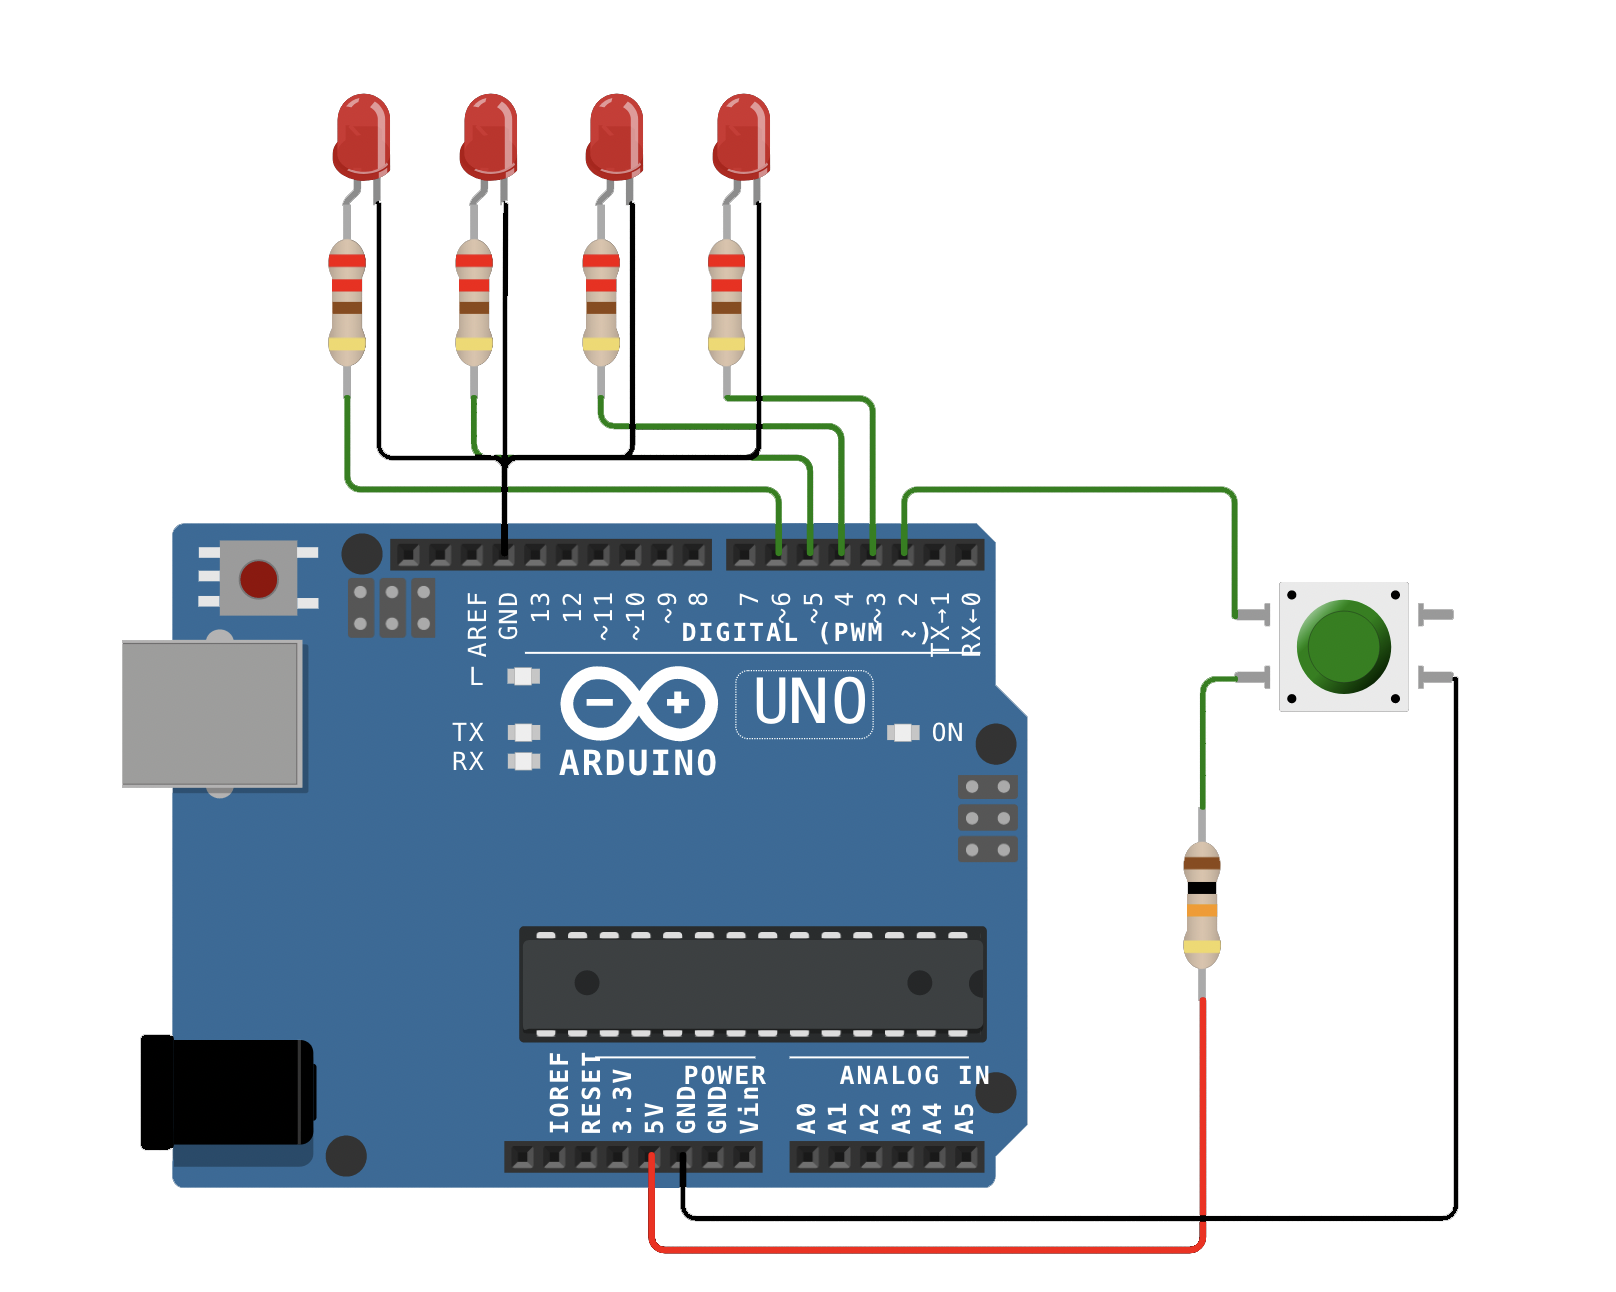
\includegraphics[width=16cm]{L1-Circuit.png}
    \caption{مدار آزمایش اول}
    \label{fig:l1circ}
\end{figure}

\pagebreak


